\documentclass[a4paper, 12pt]{article}

\usepackage[T1]{fontenc}
\usepackage[utf8]{inputenc}
\usepackage[spanish, mexico]{babel}
\usepackage[style=mexican]{csquotes}
\usepackage[margin=2cm,top=2cm,includefoot]{geometry}
\usepackage[spanish, ruled, linesnumbered, lined]{algorithm2e}
\usepackage{amsmath, amsfonts, amssymb, amsthm, amsbsy, cancel}
\usepackage{microtype, parskip}
\usepackage{float, graphicx, subcaption}
\usepackage{circuitikz, tikz, pgfplots}
\usepackage{xcolor}
\usepackage{array, booktabs, multicol, multirow, tabularx}
\usepackage{hyperref, url}
\usepackage{siunitx}
\usepackage{tcolorbox}
\usepackage[style=ieee]{biblatex}
%definir el estilo de lapagina
\usepackage{fancyhdr}

%variables de color
\definecolor{greenPortada}{HTML}{69A84F}
\definecolor{lineCabecera}{HTML}{5DADE2}

%cabecera
\setlength{\headheight}{40pt}
\pagestyle{fancy}
\fancyhf{}
\renewcommand{\headrulewidth}{3pt}
\renewcommand{\headrule}{\hbox to \headwidth{\color{lineCabecera}\leaders\hrule height \headrulewidth\hfill}}

%variables globales
\newcommand{\esquema}{imag/fourierA.png}
\newcommand{\suma}{imag/fourierB.png}
\newcommand{\resta}{imag/graffA1.png}
\newcommand{\equal}{imag/graffA2.png}
\newcommand{\less}{imag/graffA3.png}
\newcommand{\mayor}{imag/graffA4.png}



\pgfplotsset{compat=1.18}
\SetKwIF{SSi}{EnOtroCasoSi}{EnOtroCaso}{si}{entonces}{si no, si}{si no}{fin si}

\hypersetup{
    breaklinks=true,
    colorlinks=true,
    citecolor=black,
    filecolor=magenta,
    linkcolor=black, 
    urlcolor=cyan
}

\title{Simulación de un sistema con suma,resta y comparación de 2 palabras de 4 bits}

\author{Palomino Alfonso Edgar.\\Universidad Nacional Autónoma de México.\\Facultad de Estudios Superiores Cuatitlán.}
\date{\today}
\cfoot{\thepage}

\begin{document}
    \maketitle  
    \vspace{2ex}

    \section{Introducción}
    La suma, la resta y la comparación son operaciones aritméticas básicas que se utilizan en una amplia gama de aplicaciones de ingeniería y ciencias de la computación. En este reporte, se presenta el diseño y la implementación de un sistema digital que realiza estas operaciones sobre dos palabras de 4 bits.
    El sumador y el restador se basan en un diseño tradicional de acarreo completo. El comparador se basa en un comparador de magnitud de 4 bits.
    Se tiene un funcionamiento tal que la suma llega a el número máximo de los 4 bits, mientras que para la resta se restringe los resultados a solo número positivos, por último el comparador tiene el funcionamiento solicitado. La comparación es la operación de determinar si dos números son iguales, si uno es mayor que el otro o si uno es menor que el otro.
    
    \section{Descripción del metodo}
    La solución propuesta para el sistema consiste en una entrada binaria a un sumador completo de 4 bit, el cual tiene a la salida un formato BCD, debido a que nesesitamos pasarlo a 2 display de 7 segmentos y tanto como el restador, asi como el comparador sigue esta convención, se tiene condiciona la salida de este sumador de tal manera que si es menor que nueve, solo se complementa con 0 para tener 8 bits a la salida, (4 por cada display de 7 segmentos) si es menor que 19 se le suman 6, si es menor a 29 se suman 12, siguiendo esta logica el ultimo caso tiene una suma de 18, esto sirve para segmentar en 4 bits las combinaciones nesesarias para la respresentacion en los display de 7 segmentos, la resta cuenta con el problema de que si se require tener numero negativos de 2 digitos decimales requeririamos un display extra para representar el signo, caso que no se cubre en este sistema, asi que si x > y se realiza la resta y se hace la representacion con las mismas condiciones que en la suma, para el comparador se require un cambio de logica ligero debido a que se require que se presente una G si x > y; una E si x = y; y una L si x < y, asi que que para cada caso se tiene que dar una representacion ajena a la suma y resta, esto da como resultado que en el decodificador de 7 segmento se tenga que restringir 3 combinaciones para realizar esta representación, esto se puede manejar de 2 maneras, dejar la representacion hatas 19 y usar el resto de combinaciones para hacer la representación de las letras nesesarias o dentro de la multiplexación hacer uso de diferentes codifcadores antes de pasar a los display, caso que se presenta en la simulación realizada, dando como resultado a la salida de cada "modulo" una palabra de 8 bits que se puede segmentar en 4 bits para cada display.
    La elección de que se necesita queda en el multiplexor de tal manera que si tenemos 01 realizaremos la suma de las entradas, si colocamos 10 tendremos a la salida la resta, por último el bit que es vital para la comparación es el segundo así que si tenemos \emph{X1} generamos la comparación. Por último se creó un puente para tener una mejor organización de las conexiones, lo cual solo impacta en la estética, adicional a esto se solicita que se muestra la representación decimal en display de 7 segmentos de cada una de la entradas, dando como resultado la figura~\ref{fig:top-level}

    \begin{figure}[H]
        \centering
        \includegraphics[width=\textwidth]{\esquema}
        \caption{Diseño del Top-level}
        \label{fig:top-level}
    \end{figure}

    \section{Experimentos}
    El diseño del sistemo como tal no es complejo, solo que requiere de cuestiones específicas que se tiene que solventar de una manera que hace crecer al sistema, donde si no fuera por el hecho de que se terminan encapsulando los circuitos, para crear subcircuitos, se tendría un diseño muy sucio y un desastre en la presentación final, fuera de eso solo se requieren las 16 combinaciones respectivas por entrada para verificar el correcto funcionamiento del sistema, todo lo demás queda resuelto por el sistema de manera satisfactoria al ingresar las entradas y seleccionar qué operación se quiere realizar, algunas de dichas entradas y operaciones se muestran en el Apéndice A.

    \section{Conclusión}
    El diseño de este sitema se ve limitado por cuestiones puntules pero interesantes, las cuales me llevaron a repasar los fundamentos basicos de los sistemas digitales que son importnates para comprender sistemas mas complejos, si bien no se desarrollo desde compuertas el sistema, si se require entender que es lo que se tiene en cada salida de los subsistemas, esto con la finalida de llevar a cabo la siguiente etapa del sistema, o de ditribuir, diseñar, segmentar o tratar la salida para hacer un correcto acople a el sistema siguiente, como comentario final podria refereciar el pensamiento de que no se require inventar el hilo negro ya que hay problemas que han sido estudiado por mucho tiempo y por diferentes personas, pero si se requieren bases suficientes para poder implementar soluciones ya estudiadas a nuevos problemas.

    \appendix
    \section*{Apéndice A: Resultados experimentales}
    \begin{figure}[H]
        \centering
        \includegraphics[width=\textwidth]{\suma}
        \caption{Suma}
    \end{figure}
    \begin{figure}[H]
        \centering
        \includegraphics[width=\textwidth]{\resta}
        \caption{Resta}
    \end{figure}
    \begin{figure}[H]
        \centering
        \includegraphics[width=\textwidth]{\mayor}
        \caption{X > Y}
    \end{figure}
    \begin{figure}[H]
        \centering
        \includegraphics[width=\textwidth]{\equal}
        \caption{X = Y}
    \end{figure}
    \begin{figure}[H]
        \centering
        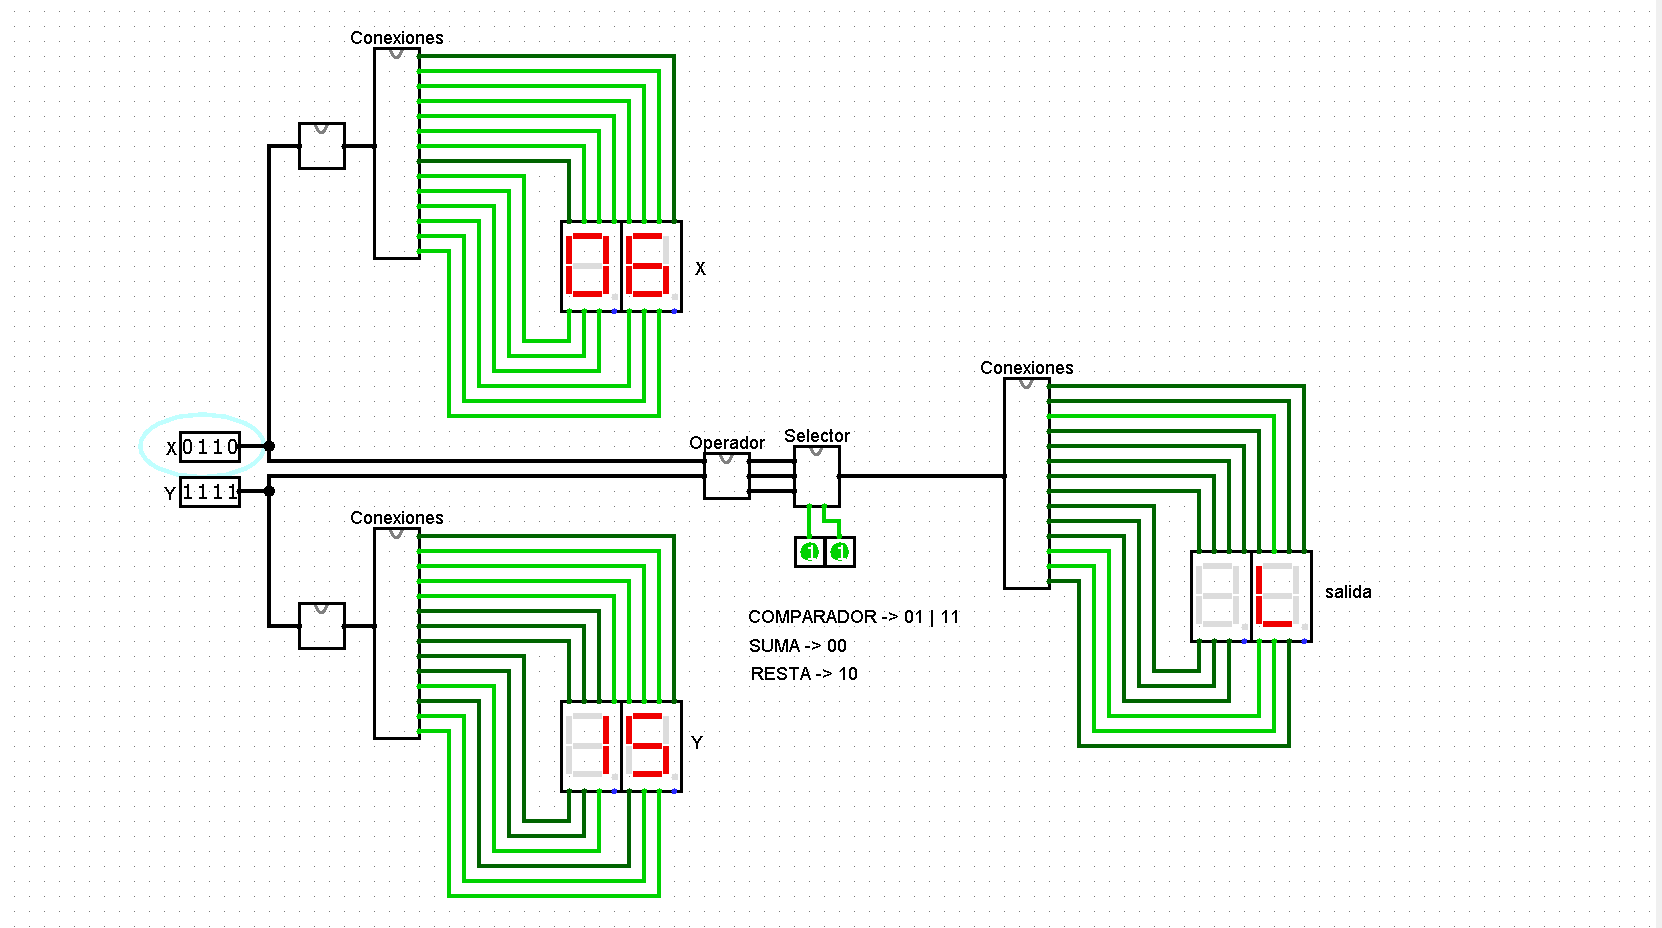
\includegraphics[width=\textwidth]{\less}
        \caption{X < Y}
    \end{figure}

\end{document}
